\documentclass[tikz,border=2mm]{standalone}
\usepackage{amsmath,braket}
\usetikzlibrary{arrows.meta,calc}

% All artwork is native TikZ. Change these colors/styles to restyle it.
\definecolor{modelblue}{HTML}{0072B2}
\definecolor{condone}{HTML}{009E73}
\definecolor{condtwo}{HTML}{E69F00}
\definecolor{condthree}{HTML}{CC79A7}
\definecolor{ink}{HTML}{3D4852}
\tikzset{
  every node/.style={font=\fontsize{9}{10.5}\selectfont,text=ink},
  heading/.style={font=\fontsize{10}{11}\selectfont\bfseries,anchor=west},
  label/.style={font=\fontsize{9}{10.5}\selectfont,align=center},
  small/.style={font=\fontsize{8}{9}\selectfont,align=center},
  flow/.style={-{Latex[length=2mm]},draw=ink!70,line width=.8pt},
  feedback/.style={flow,draw=modelblue},
  transfer/.style={feedback,dashed},
  outline/.style={draw=ink!65,line width=.65pt,rounded corners=2pt},
}

% A condition-tagged card. All bitstrings are schematic placeholders.
\newcommand{\samplecard}[5]{%
  \begin{scope}[shift={(#1,#2)}]
    \draw[outline,fill=#3!5] (-1.7,-.32) rectangle (1.7,.32);
    \fill[#3] (-1.7,-.32) rectangle (-1.62,.32);
    \node[font=\fontsize{8}{9}\selectfont,text=#3!70!black] at (0,.13) {Condition $#4$};
    \node[font=\fontsize{8}{9}\selectfont\ttfamily] at (0,-.15) {#5};
  \end{scope}}

\begin{document}
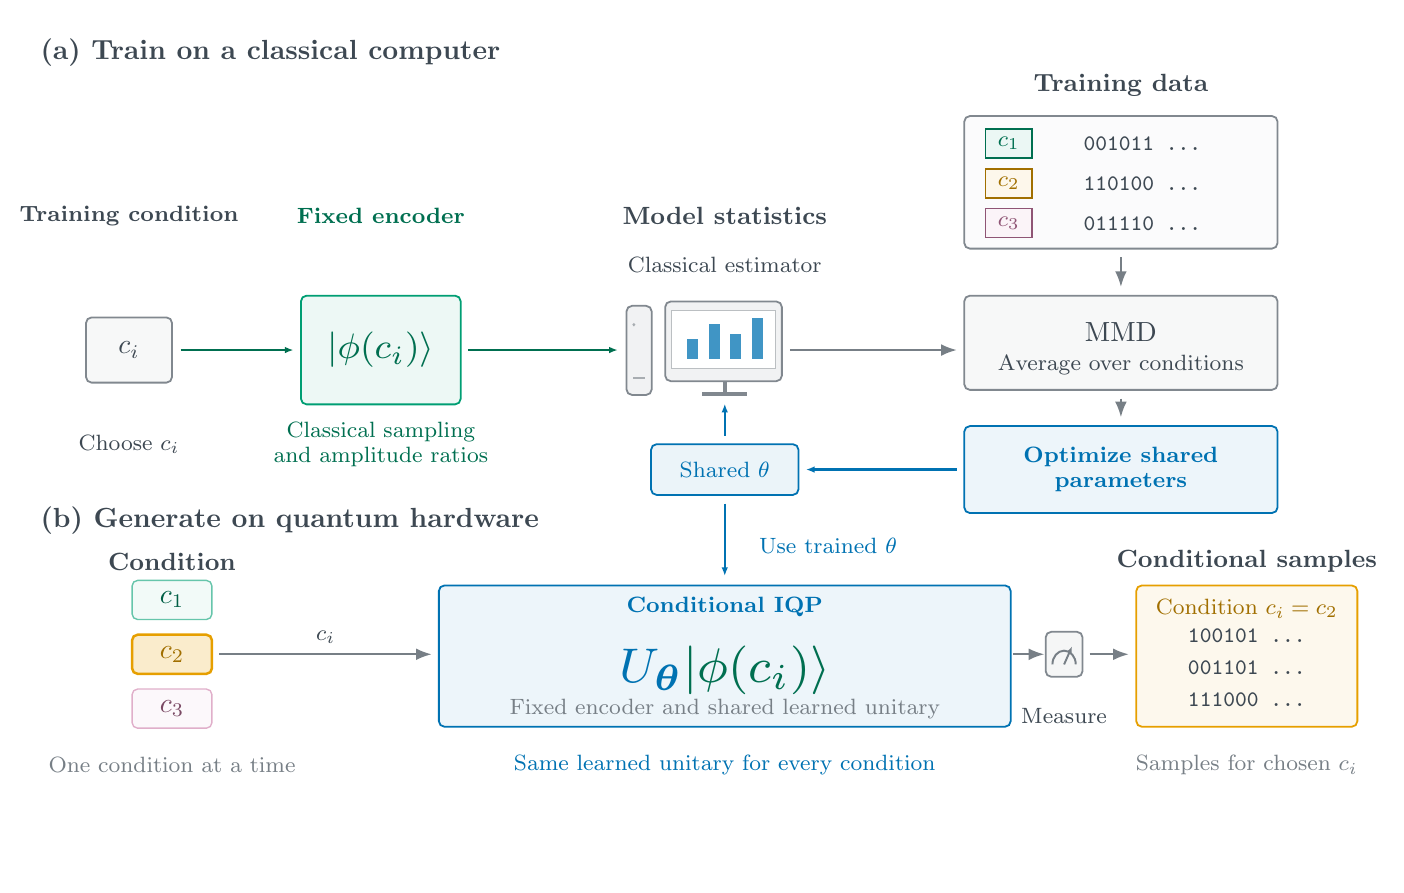
\begin{tikzpicture}[x=.78cm,y=.92cm]
\path[use as bounding box] (-.05,-.55) rectangle (21.9,11.0);

% Classical training: data and model statistics meet at the conditional MMD objective.
\node[heading] at (0,10.65) {(a) Train on a classical computer};
\node[small,font=\fontsize{8}{9}\selectfont\bfseries] at (1.6,8.4) {Training condition};
\draw[outline,fill=ink!4] (.9,6.1) rectangle (2.3,7.0);
\node[font=\fontsize{10}{11}\selectfont] at (1.6,6.55) {$c_i$};
\node[small] at (1.6,5.25) {Choose $c_i$};
\node[font=\fontsize{8}{9}\selectfont\bfseries,text=condone!70!black] at (5.7,8.4) {Fixed encoder};
\draw[outline,draw=condone,fill=condone!7] (4.4,5.80) rectangle (7.0,7.30);
\node[font=\fontsize{8}{9}\selectfont,text=condone!70!black] at (5.7,6.55) {\scalebox{1.6}{$\ket{\phi(c_i)}$}};
\node[small,text=condone!70!black] at (5.7,5.25) {Classical sampling\\and amplitude ratios};
\node[label] at (11.3,8.4) {\textbf{Model statistics}};
\draw[outline,fill=ink!7] (9.70,5.93) rectangle (10.11,7.16);
\fill[ink!45] (9.82,6.90) circle (.025);
\draw[ink!45,line width=.6pt] (9.81,6.16) -- (10.00,6.16);
\draw[outline,fill=ink!7] (10.33,6.12) rectangle (12.23,7.22);
\draw[fill=white,draw=ink!35,line width=.4pt] (10.43,6.30) rectangle (12.13,7.10);
\draw[ink!65,line width=1.4pt] (11.30,5.94) -- (11.30,6.12);
\draw[ink!65,line width=1.4pt] (10.93,5.94) -- (11.67,5.94);
\foreach \xx/\hh in {10.69/.27,11.04/.48,11.39/.34,11.74/.56} {\fill[modelblue!75] (\xx,6.43) rectangle ++(.18,\hh);}
\node[small] at (11.3,7.72) {Classical estimator};
\node[label] at (17.75,10.20) {\textbf{Training data}};
\draw[outline,fill=ink!2] (15.2,7.95) rectangle (20.3,9.78);
\foreach \yy/\col/\tag/\bits in {9.40/condone/c_1/{001011 ...},8.85/condtwo/c_2/{110100 ...},8.30/condthree/c_3/{011110 ...}} {
  \draw[draw=\col!70!black,fill=\col!8,line width=.5pt] (15.55,\yy-.20) rectangle (16.3,\yy+.20);
  \node[font=\fontsize{8}{9}\selectfont,text=\col!70!black] at (15.925,\yy) {$\tag$};
  \node[font=\fontsize{8}{9}\selectfont\ttfamily] at (18.1,\yy) {\bits};
}
\draw[outline,fill=ink!4] (15.2,6.0) rectangle (20.3,7.3);
\node[font=\fontsize{10}{11}\selectfont] at (17.75,6.8) {MMD};
\node[small] at (17.75,6.35) {Average over conditions};
\draw[flow] (17.75,7.83) -- (17.75,7.42);
\draw[draw=condone!70!black,-{Latex[length=1.1mm]},line width=.7pt] (2.44,6.55) -- (4.28,6.55);
\draw[draw=condone!70!black,-{Latex[length=1.1mm]},line width=.7pt] (7.12,6.55) -- (9.56,6.55);
\draw[flow] (12.36,6.55) -- (15.08,6.55);
\draw[outline,draw=modelblue,fill=modelblue!7] (15.2,4.3) rectangle (20.3,5.5);
\node[small,font=\fontsize{8}{9}\selectfont\bfseries,text=modelblue] at (17.75,4.9) {Optimize shared\\parameters};
\draw[flow] (17.75,5.88) -- (17.75,5.62);
\draw[outline,draw=modelblue,fill=modelblue!8] (10.1,4.55) rectangle (12.5,5.25);
\node[small,text=modelblue] at (11.3,4.9) {Shared $\theta$};
\draw[draw=modelblue,-{Latex[length=1.1mm]},line width=.8pt] (15.08,4.9) -- (12.62,4.9);
\draw[draw=modelblue,-{Latex[length=1.1mm]},line width=.8pt] (11.3,5.37) -- (11.3,5.81);
\draw[draw=modelblue,-{Latex[length=1.1mm]},line width=.8pt] (11.3,4.43) -- (11.3,3.43);
\node[small,text=modelblue,anchor=west] at (11.7,3.85) {Use trained $\theta$};

% One explicit generation call, shown with an example selected condition.
\node[heading] at (0,4.20) {(b) Generate on quantum hardware};
\node[label] at (2.3,3.63) {\textbf{Condition}};
\foreach \yy/\col/\tag in {3.10/condone/c_1,1.60/condthree/c_3} {
  \draw[draw=\col!60,fill=\col!5,line width=.5pt,rounded corners=2pt]
    (1.65,\yy-.27) rectangle (2.95,\yy+.27);
  \node[font=\fontsize{10}{11}\selectfont,text=\col!60!black] at (2.3,\yy) {$\tag$};
}
\draw[draw=condtwo,fill=condtwo!20,line width=.9pt,rounded corners=2pt]
  (1.65,2.08) rectangle (2.95,2.62);
\node[font=\fontsize{10}{11}\selectfont,text=condtwo!70!black] at (2.3,2.35) {$c_2$};
\node[small,text=ink!70] at (2.3,.82) {One condition at a time};
\draw[flow] (3.07,2.35) -- node[above,small] {$c_i$} (6.53,2.35);

\draw[outline,draw=modelblue,fill=modelblue!7] (6.645,1.35) rectangle (15.955,3.30);
\node[font=\fontsize{8}{9}\selectfont\bfseries,text=modelblue] at (11.3,3.01) {Conditional IQP};
\node[font=\fontsize{8}{9}\selectfont,text=modelblue] at (11.3,2.13)
  {\scalebox{2.2}{$U_{\boldsymbol\theta}\textcolor{condone!70!black}{\ket{\phi(c_i)}}$}};
\node[small,text=ink!70] at (11.3,1.60) {Fixed encoder and shared learned unitary};
\node[small,text=modelblue] at (11.3,.82) {Same learned unitary for every condition};
\draw[flow] (15.99,2.35) -- (16.505,2.35);
\draw[outline,draw=ink!65,fill=ink!5] (16.525,2.04) rectangle (17.125,2.66);
\draw[ink!70,line width=.7pt] (16.635,2.21) arc[start angle=180,end angle=0,radius=.19];
\draw[ink!70,line width=.7pt,-{Latex[length=.8mm]}] (16.825,2.21) -- (16.955,2.46);
\node[small] at (16.825,1.50) {Measure};
\draw[flow] (17.24,2.35) -- (17.88,2.35);

\node[label] at (19.8,3.63) {\textbf{Conditional samples}};
\draw[outline,draw=condtwo,fill=condtwo!7] (18,1.35) rectangle (21.6,3.30);
\node[small,text=condtwo!70!black] at (19.8,2.98) {Condition $c_i=c_2$};
\node[font=\fontsize{8}{9}\selectfont\ttfamily] at (19.8,2.60) {100101 ...};
\node[font=\fontsize{8}{9}\selectfont\ttfamily] at (19.8,2.16) {001101 ...};
\node[font=\fontsize{8}{9}\selectfont\ttfamily] at (19.8,1.72) {111000 ...};
\node[small,text=ink!70] at (19.8,.82) {Samples for chosen $c_i$};
\end{tikzpicture}
\end{document}
